%!TEX root = thesis.tex

\chapter{Grundlagen} % (fold)
\label{cha:grundlagen}

Grundlagen mit den bisherigen Quellen \citealt{hilton2013}.

In diesem Kapitel werden die grundlegenden Techniken zur Webseiten-Entwicklung mit dem Play-Framework vorgestellt werden.
Dabei wird dafür benötigtes Hintergrundwissen bereitgestellt und erklärt, welche Werkzeuge benötigt werden.
Schließlich werden durch die Entwicklung einer kleinen Anwendung die einzelnen Komponenten erklärt.
Es werden hierbei in erster Linie die Komponenten vorgestellt, die für die Entwicklung von Real-Time-Web-Anwendungen unbedingt notwendig sind.


\section{Vorbereitung} % (fold)
\label{sec:vorbereitung}

Bevor auf die eigentliche Arbeit mit dem Play-Framework eingegangen wird, müssen einige vorbereitende Dinge geklärt werden. In diesem Abschnitt geht es darum, wie die Entwicklungsumgebung aufgesetzt wird, mit welcher Version der eingesetzten Software gearbeitet wird und wie sich das Play-Framework installieren lässt.

\subsection{Entwicklungsumgebung} % (fold)
\label{sub:entwicklungsumgebung}

Es kann entweder mit einem einfachen Text-Editor entwickelt werden, oder auch mit einer IDE (integrated development environment).
Für die einzelnen Programme können teilweise Plugins heruntergeladen werden, die beispielsweise code completion oder syntax highlighting für Play-spezifische Funktionalitäten bereitstellen.

Für \textbf{Eclipse} Indigo und Juno kann die Scala IDE heruntergeladen werden.
Diese IDE ist für die Entwicklung von Scala-Anwendungen mit Eclipse notwendig.
Des weiteren existiert für die Scala IDE ein Plugin für das Play-Framework, das nach Installation der Scala IDE über die gleiche Quelle, wie auch die Scala IDE installiert werden kann (siehe Abb.~\ref{fig:scala-ide-plugin-installation}).

% 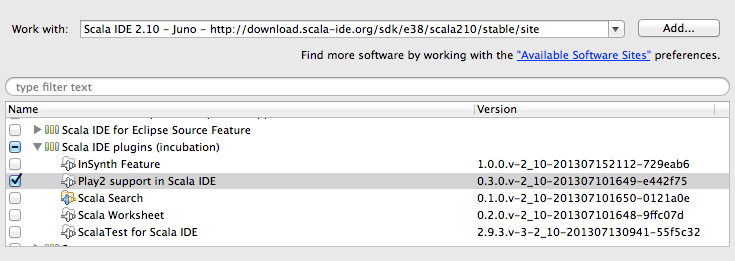
\includegraphics[width=\linewidth]{scala-ide-plugin-installation.png}
\begin{figure}[h]
\centering
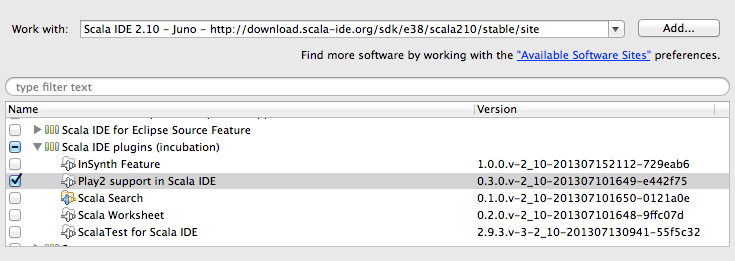
\includegraphics[width=\textwidth]{scala-ide-plugin-installation.png}
\caption{Installation des Play-Plugins für die Scala IDE}
\label{fig:scala-ide-plugin-installation}
\end{figure}


Beispiel Sublime Text 2.

Als IDE wird hier IntelliJ IDEA 12 Community Edition verwendet.
Nach dem Anlegen des Play-Projekts auf der Kommandozeile muss ein mal der Befehl \lstinline|play idea| ausgeführt werden.
Wenn man sich bereits in der Play-Eingabemaske befindet, muss man nur \lstinline|idea| ausführen.
Eine umfangreiche Liste für weitere IDEs ist bei \citealt{ide}~\footnote{\url{http://www.playframework.com/documentation/2.1.1/IDE}} zu finden.

% subsection entwicklungsumgebung (end)

% section vorbereitung (end)


\subsection{Software-Version} % (fold)
\label{sub:software_version}

% subsection software_version (end)


\subsection{Installation} % (fold)
\label{sub:installation}

% subsection installation (end)


% chapter grundlagen (end)